\section{Итоговая проверка и повреждения на новых миссиях}\label{sec:stageg}
Все части этого этапа вместе с порогами записаны до прогонов (этап G). Места проверки те же, кварталы Токио и Казани, но 300
миссий новые: новые расстановки, тексты, примерные точки и отказы. Ничего в системе на них не настраивалось.

\paragraph{Итоговая проверка (G2).} В таблице~\ref{tab:g2} система работает одна (текст оператора разбирает модель F3b, на
вопросы дрона никто не отвечает), а рядом та же система с обычным рефлексом вместо ядра чувств, на тех же 300 миссиях. Главный
результат проекта повторился на новом наборе и стал сильнее: без ядра касаются неподвижного 14,7\,\% миссий, с ядром 4,3\,\%
(парная разница $-10{,}3$ процентного пункта\ci{-14{,}7}{-6{,}0}; $-0{,}61$\ci{-0{,}92}{-0{,}35} касания на миссию). Впервые
ядро снизило и попадания атакующих птиц ($-0{,}19$\ci{-0{,}33}{-0{,}06} на миссию с атакой), а система с ядром выполнила больше
шагов ($+0{,}038$\ci{0{,}008}{0{,}070}). Правило безопасности, записанное заранее, не выполнено: без помощи оператора дрон коснулся не
той цели в 3 миссиях из 300, это 1,0\,\% с верхней бутстрэп-границей 2,3\,\% (точная граница Клоппера--Пирсона 2,9\,\%) при требуемых 2\,\%. Рис.~\ref{fig:lesion} ставит это повторение рядом
с первым опытом с повреждением.

\begin{table}[t]
\centering\small
\caption{Итоговая проверка на 300 новых миссиях в незнакомых местах (G2). Миссии одни и те же для обоих вариантов; в скобках
95\,\% бутстрэп-интервалы по миссиям. Разница парная.}
\label{tab:g2}
\setlength{\tabcolsep}{3.5pt}
\begin{tabular}{@{}lccc@{}}
\toprule
 & Ядро чувств (один) & Обычный рефлекс & Разница \\
\midrule
Миссий с касанием неподвижного & \textbf{4,3\,\%}\ci{2{,}3}{6{,}7} & 14,7\,\%\ci{10{,}7}{18{,}7} & $-10{,}3$\ci{-14{,}7}{-6{,}0}\,п.п. \\
Касаний неподвижного на миссию & & & $-0{,}61$\ci{-0{,}92}{-0{,}35} \\
Попаданий на миссию с атакой & & & $-0{,}19$\ci{-0{,}33}{-0{,}06} \\
Выполнено шагов & 0,301\ci{0{,}254}{0{,}348} & 0,257\ci{0{,}214}{0{,}304} & $+0{,}038$\ci{0{,}008}{0{,}070} \\
Выполнено миссий целиком & 0,287\ci{0{,}233}{0{,}340} & 0,253\ci{0{,}207}{0{,}303} & $+0{,}033$\ci{0{,}003}{0{,}063} \\
Не та цель (правило до 2\,\%) & 1,0\,\%\ci{0}{2{,}3} & 2,3\,\%\ci{0{,}7}{4{,}0} & $-1{,}3$\ci{-3{,}0}{-0{,}3}\,п.п. \\
\bottomrule
\end{tabular}
\end{table}

\begin{figure}[t]
\centering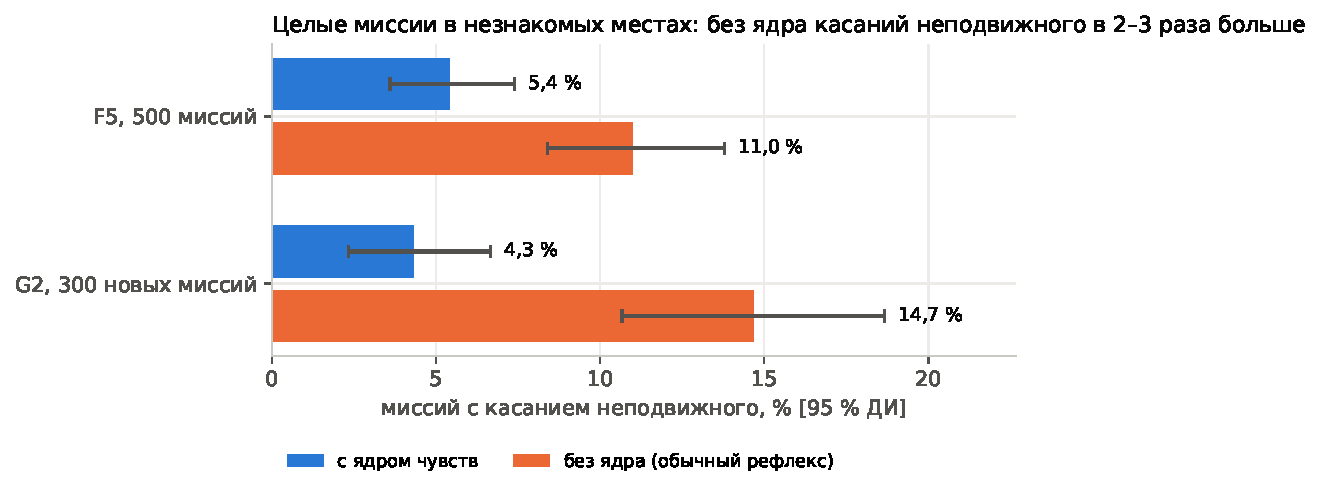
\includegraphics[width=.92\linewidth]{fig_missions_lesion_ru.pdf}
\caption{Целые миссии в незнакомых настоящих местах с ядром чувств и с обычным рефлексом вместо него. F5~--- первый опыт с
повреждением (500 миссий), G2~--- 300 новых миссий. Интервалы: 95\,\% бутстрэп по миссиям.}
\label{fig:lesion}
\end{figure}

\paragraph{Один и с оператором.} По действиям дрон в одиночку выполнил пролёт в 0,49 шагов, посадку в 0,44, осмотр в 0,30,
захват крюком в 0,29, сброс на парашюте в 0,22 и влёт в ангар в 0,14. Большая часть неудач~--- это отказы по замыслу: если описание
не выделяет один объект, дрон не трогает ни один. Приложение задумано для работы с человеком, который проверяет разбор и отвечает
на вопросы дрона, поэтому первые 200 миссий мы пролетели ещё раз именно так. Оператор в симуляции получает верный разбор и на
вопрос выбирает того кандидата, который стоит у задуманного объекта. На 182 миссиях, закончившихся до предела времени прогона
(18 ещё летели), дрон с оператором выполнил 0,56 шагов против 0,29 в одиночку на тех же миссиях (парная разница
$+0{,}27$\ci{0{,}20}{0{,}33}) и 0,54 миссий целиком против 0,29 (рис.~\ref{fig:actions}). Большинству миссий вопрос вообще не
понадобился (медиана 0, 90-й процентиль 1). У помощи есть цена: теперь дрон долетает каждый шаг до конца, и миссий с касанием
неподвижного стало 10,4\,\% вместо 3,8\,\% ($+6{,}6$\ci{2{,}7}{10{,}4} п.п.). Не той цели он коснулся в 4 миссиях (2,2\,\%), две
из них~--- это те же ошибки, что и в одиночку, без вопроса. В трёх миссиях, где ни один кандидат не был целью, дрон спрашивал снова и
снова (от 131 до 541 раза), и приложению там нужен предел.

\begin{figure}[t]
\centering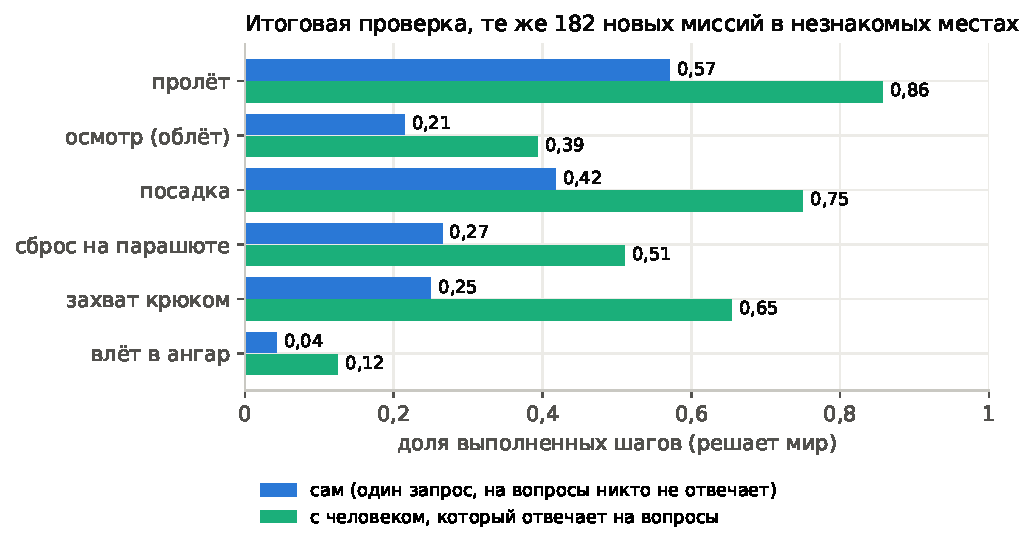
\includegraphics[width=.8\linewidth]{fig_actions_ru.pdf}
\caption{Выполненные шаги по действиям на тех же 182 новых миссиях: дрон один и дрон с человеком, который проверяет разбор и
отвечает на вопросы. Засчёт по миру: на что сел, куда упал груз, что висит на крюке.}
\label{fig:actions}
\end{figure}

\paragraph{Дверь ангара (G1).} Влёт в ангар был самым слабым действием, и одна разобранная неудача показала, что искатель двери
принял щель в задней стене за дверь. Мы попробовали правило строже: проём считается, только если сквозь него лидар видит пол
ангара. Когда дрон ставили на окружность вокруг 90 ангаров, старый искатель нашёл верную дверь у 74 из 76 открытых ангаров и ни
одной двери у 14 закрытых; новый нашёл 72, пропустил 4 и увидел дверь у 3 закрытых. В полёте, с верным разбором и человеком,
который отвечает на вопросы дрона, новый искатель влетел в 1 ангар из 38 полётов, старый в 6 из 37. Пока дрон облетает ангар,
его собственная оценка положения уплывает и размазывает точки стен по коробке. По правилу, записанному заранее, остаётся старый
искатель.

\paragraph{Медленные чувства в тяжёлых миссиях (G3).} Медленные чувства («я потерялся», «мало сил») в коротких миссиях F5 почти
не срабатывали, поэтому этап G проверил их там, где они должны быть нужны. В 120 тяжёлых миссиях на местах проверки заряд при
взлёте от 30 до 65\,\%, в 60\,\% миссий батарея холодная, ветер от 3 до 9\,м/с, GPS пропадает (в 47 из 99 пролетевших миссий) или подменяется (в 26), есть атаки птиц,
и возврат домой обязателен. Разбор верный, так что проверяется только медленный слой. Пять вариантов летели одни и те же миссии:
чувства ядра; сырая телеметрия с порогами вместо них, которая сравнивает заряд с энергией на дорогу домой; без медленного слоя; и
без каждого чувства по очереди. Из-за предела времени успели 99 миссий (98 у трёх вариантов; рис.~\ref{fig:slow}).

С чувствами ядра батарея села в воздухе в 29\,\% миссий, без медленного слоя тоже в 29\,\% (парная разница
$0{,}0$\ci{-7{,}1}{7{,}1} п.п.). Первое ожидание, что медленный слой предотвращает такие падения, не подтвердилось. Сырая
телеметрия справилась лучше: 16\,\% падений ($-13{,}1$\ci{-21{,}2}{-5{,}1} п.п. против чувств) и больше посадок дома (63 против
52\,\%, $+11{,}1$\ci{5{,}1}{18{,}2}). Заплатила она меньшим числом целых миссий ($-0{,}040$\ci{-0{,}081}{-0{,}010}), потому что
вдвое чаще поворачивала домой раньше времени. Значит, H6 не подтверждена, как мы и записали заранее: чувство «мало сил» обучено
на 40-секундных эпизодах и не знает расстояния до дома, а правило телеметрии умножает расход на это расстояние. Чувство
действовало (с ним дрон раньше времени поворачивал домой в 13\,\% миссий, без него ни разу), но падений меньше не стало
($0{,}0$\ci{-6{,}1}{6{,}1}). Без «я потерялся» не изменились ни падения, ни возвраты. Одно наблюдение не планировалось: без
«я потерялся» дрон реже касался неподвижного ($-0{,}22$\ci{-0{,}43}{-0{,}06} касания на миссию). Для настоящего аппарата вывод
простой. Запас энергии должно считать явное правило по расстоянию и расходу, а не выученное чувство.

\begin{figure}[t]
\centering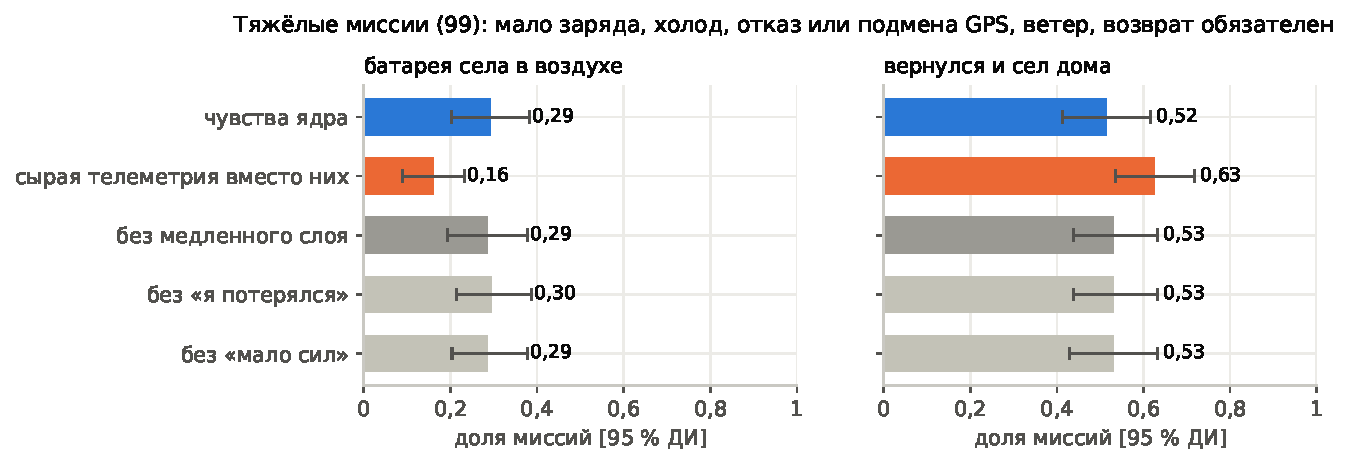
\includegraphics[width=\linewidth]{fig_slow_ru.pdf}
\caption{Тяжёлые миссии (G3), одни и те же для всех вариантов. Слева миссии, где батарея села в воздухе, справа миссии, которые
кончились посадкой дома. Сырая телеметрия с правилом «энергия до дома» лучше выученных медленных чувств; без медленного слоя или
без одного чувства ничего не меняется. Интервалы: 95\,\% бутстрэп по миссиям.}
\label{fig:slow}
\end{figure}

\paragraph{Ложные и запоздавшие чувства (G4).} Пациенты Дамасио подсказывают ещё два повреждения: чувство, которое срабатывает,
когда ничего нет, и чувство, которое приходит слишком поздно. На первых 100 миссиях итоговой проверки мы ещё дважды пролетели
полную систему. В первом варианте маркер «продолжать» показывал опасность в пустом небе на 1\,с в случайные моменты, примерно раз
в 20\,с; во втором маркеры видели мир на 0,3\,с позже. Ложные тревоги добавили 24 перехвата на миссию\ci{19}{29} и не стоили
шагов ($+0{,}015$\ci{-0{,}05}{0{,}08}), но миссий с касанием неподвижного стало 9\,\% вместо 4\,\% ($+5{,}0$\ci{0{,}0}{10{,}0}
п.п.). Лишний отворот на улице сам может кончиться стеной. Мы ждали меньше шагов и не меньше касаний; вторая половина ожидания
сбылась, первая нет. Запоздание на 0,3\,с почти ничего не изменило: миссий с касанием неподвижного $+3{,}0$\ci{-1{,}0}{8{,}1}
п.п., так что ожидаемый рост не подтвердился. Маркеры смотрят на 2\,с вперёд, и задержка в 0,3\,с мала против этого горизонта.

\subsection{К настоящему аппарату: мозг на автопилоте PX4}\label{sec:px4}
Дрон летает на автопилоте, а не на регуляторе нашего симулятора. Мы написали мост MAVLink, который даёт неизменённому мозгу миссии
тот же интерфейс на настоящем автопилоте (PX4 \citep{meier2015px4} или ArduPilot): телеметрия на вход, заданные скорости на выход с частотой 20\,Гц,
перевод систем координат, сторожевой таймер, который держит точку, если мозг опаздывает, и собственные защиты автопилота под всем
этим. Затем мы провели 12 миссий (посадка, сброс, захват, осмотр, пролёт, цели на земле) на программной сборке PX4 с её моделью
квадрокоптера SIH, каждые 0,1\,с ставя наш мир в оценённое PX4 положение, чтобы лидар, камера и засчёт оставались нашими. Мост
сработал механически: PX4 включал моторы, взлетал, выполнял команды мозга, садился, снова включался и отказывался взлетать, когда
отказывали его датчики. Успех миссий не перенёсся: 1 из 12 миссий с PX4 против 7 из 12 с нашим регулятором на тех же миссиях, и
удержание точки собственным контуром положения PX4 в точных фазах ничего не изменило. PX4 отрабатывает команды скорости мозга с
медианной ошибкой от 0,8 до 1,3\,м/с, и миссии шли примерно вдвое дольше. Тайм-ауты, скорости и точные фазы мозга настроены на нашем
регуляторе; до любого полёта их нужно перенастроить и заново проверить на настоящем автопилоте.
